%%%%%% PART 1%%%%%%%

\begin{frame}
\frametitle{Model problem and settings: contact between two membranes}
\vspace{-1.7 cm}
\begin{equation*}
\mbox{Find} \ u_1, u_2, \lambda \ \mbox{such that} \quad
\dps
\left\lbrace\begin{array}{llccc}
\dps -\mu_1 \Delta u_1-\lambda = f_1 \qquad \mbox{in} \quad \Omega, \\
\dps -\mu_2 \Delta u_2+\lambda = f_2 \qquad \mbox{in} \quad \Omega,\\
\textcolor{electricpurple}{u_1-u_2 \geq 0}, \quad 
\textcolor{carmine}{\lambda \geq 0}, \quad \dps (\textcolor{electricpurple}{u_1-u_2})\textcolor{carmine}{\lambda}=0 \quad \mbox{in} \quad \Omega, \hspace{0.2 cm}\\
\dps u_1=g_1, \ u_2=g_2  \qquad \mbox{on} \quad\partial \Omega.
\end{array}
\right.
\end{equation*}
\vspace{-0.8 cm}
\begin{figure}
\begin{subfigure}[normal]{0.44\textwidth} 
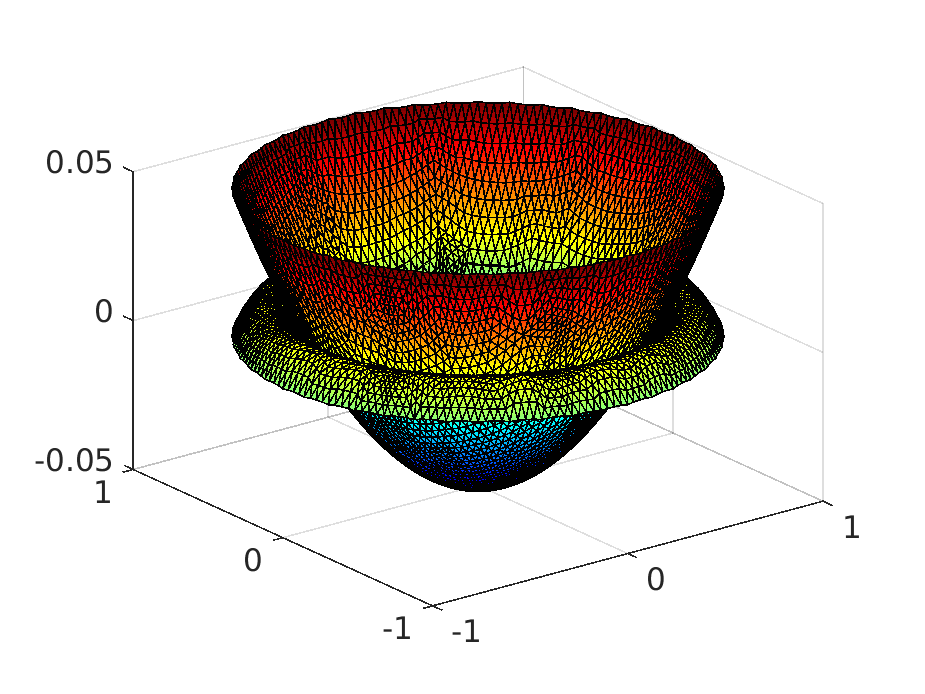
\includegraphics[width=\textwidth]{fig_article_chap_1/fig_membrane_cv.eps}    
\end{subfigure}
\qquad
\begin{subfigure}[normal]{0.44\textwidth}
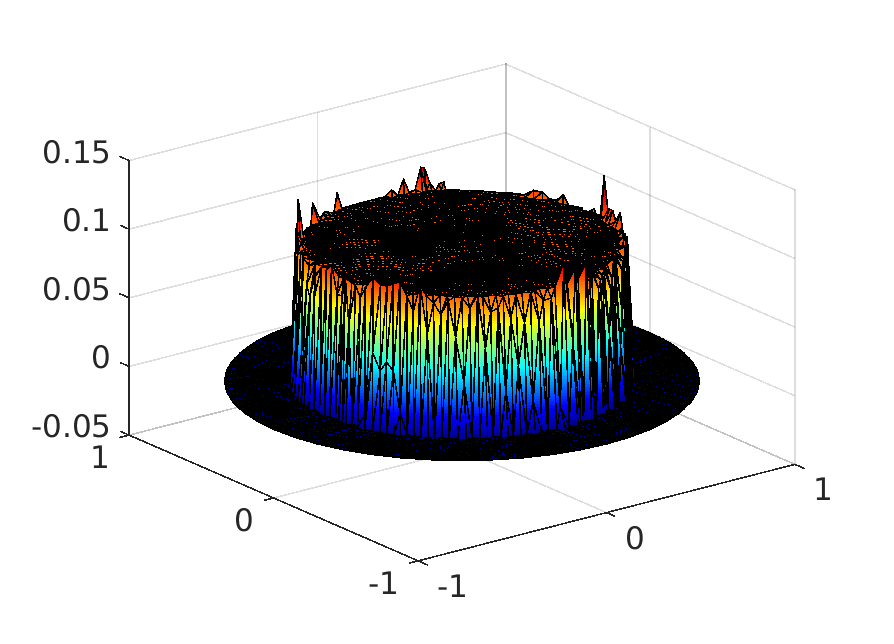
\includegraphics[width=\textwidth]{fig_article_chap_1/fig_lambda_cv.eps}     
\end{subfigure}
\end{figure}
\vspace*{-4.4cm}\hspace*{1.5 cm}$u_1$ \hspace{8 cm} $\lambda$\\
\vspace*{0.7cm}\hspace*{1.5 cm}$u_2$\\
\end{frame}
%%%%%
\begin{frame}
\frametitle{Continuous problem}
\begin{itemize}
\item $H_{g_{\alpha}}^1(\Omega)\hspace{-0.1 cm} =\hspace{-0.1 cm} \left\{u\in H^1(\Omega), \hspace{0.1 cm} u=g_{\alpha} \hspace{0.1 cm} \mbox{on} \hspace{0.1 cm} \partial \Omega\right\}$ \quad $\Lambda=\left\{\chi\in L^2(\Omega), \: \textcolor{carmine}{\chi \geq 0} \: \mbox{a.e.} \hspace{0.1 cm} \mbox{in} \ \Omega\right\}$
\end{itemize}
\textbf{Saddle point type weak formulation:}
For $(f_1,f_2)\in \left[L^2(\Omega)\right]^2$ and $g > 0$ find $(u_1,u_2,\lambda)\in H_{g_1}^1(\Omega) \times H_{g_2}^1(\Omega) \times \Lambda$ such that
\begin{equation*}
\begin{split}
& \dps \sum_{\ialf=1}^2 \mu_\ialf \left(\nab u_\ialf,\nab v_\ialf\right)_{\Omega} - \left(\lambda,v_1-v_2\right)_{\Omega} = \sum_{\ialf=1}^2\left(f_\ialf,v_\ialf\right)_{\Omega} \quad \forall (v_1,v_2) \in \left[H_0^1(\Omega)\right]^2 \\
& \left(\chi - \textcolor{carmine}{\lambda},\textcolor{electricpurple}{u_1-u_2}\right)_{\Omega} \geq 0 
\quad \forall \chi \in \Lambda 
\end{split}
 \tag{$\textcolor{electricpurple}{\mathrm{S}}$}
\end{equation*}
\invisible<1>{
\hspace{4.5 cm}\textcolor{cadmiumgreen}{\textbf{equivalent to}}\\
\invisible<2>{
\textbf{Variational inequality:}
\begin{itemize}
\item $\Kg:= \left\{(v_1,v_2)\in H_{g_1}^1(\Omega)\times H_{g_2}^1(\Omega),\: \textcolor{electricpurple}{v_1-v_2 \geq 0} \; \; \mbox{a.e.} \ \mbox{in} 
\hspace{0.1 cm} \Omega \right\}$ \textcolor{midnightblue}{\textbf{convex}}
\end{itemize}
\begin{equation*}
\mbox{Find} \ \bu=\left(u_1,u_2\right) \in \Kg \ \mbox{s.t.} \ \dps \sum_{\ialf=1}^2 \mu_\ialf \left(\nab u_\ialf,\nab \left(v_\ialf-u_\ialf\right)\right)_{\Omega} \geq \sum_{\ialf=1}^2\left(f_\ialf,v_\ialf-u_\ialf\right)_{\Omega} \quad \forall \bv \in \Kg  \tag{$\textcolor{electricpurple}{\mathrm{R}}$}
\end{equation*}
\invisible<3>{
}}}
\end{frame}
%%%%%
\begin{frame}
\textcolor{red}{\textbf{For any $p \geq 1$}}
\\
\frametitle{The finite element method}
\textcolor{cadmiumgreen}{\textbf{Spaces for the discretization:}}\\
$X_{g_{\alpha}h}^p=\left\{v_h \in \mathcal{C}^0(\overline{\Omega}),  {v_h}_{|K} \in \Pp (K), \ \forall K \in {\mathcal{T}}_h, \hspace{0.2 cm} v_h=g_\alpha \hspace{0.2 cm} \mbox{on} \hspace{0.2 cm} \partial \Omega\right\}$\\
\vspace*{0.3 cm}
$\Xzerohp =\left\{v_h \in \calC^0(\overline{\Omega}); \ {v_h}|_{K} \in \Pp (K), \ \forall K \in \Th, \hspace{0.2 cm} v_h=0 \hspace{0.2 cm} \mbox{on} \hspace{0.2 cm} \partial \Omega \right\}$
\\
\vspace*{0.3 cm}
$\dps \Kghp=\left\{(\vunh,\vdeuxh) \in X_{g_1 h}^p \times X_{g_2 h}^p, \ \textcolor{electricpurple}{\vunh(\xl)-\vdeuxh(\xl)} \geq 0 \ \ \forall \xl \in \Vdp \right\} \textcolor{red}{\not \subset \Kg \quad \forall p \geq 2}$\\
\vspace*{0.2 cm}
\invisible<1>{
\textcolor{cadmiumgreen}{\textbf{Discrete variational inequality:}} find $\dps \uh=(\uunh,\udeuxh) \in \Kghp$ such that
\begin{equation*}
\dps \sum_{\ialf=1}^2 \mu_\ialf \left(\nab u_{\ialf h},\nab \left(v_{\ialf h}-u_{\ialf h}\right)\right)_{\Omega} \geq \sum_{\ialf=1}^2\left(f_\ialf,v_{\ialf h}-u_{\ialf h}\right)_{\Omega} \quad \forall \bv_h = (v_{1h},v_{2h})\in ~\Kghp \quad \textcolor{electricpurple}{(\mathrm{DR})}
\end{equation*}
\begin{center}
\textcolor{midnightblue}{Well-posed problem (Lions--Stampacchia)}
\end{center}
\invisible<2>{
\textcolor{midnightblue}{\textbf{Resolution techniques:}}
\footnotesize{Projected Newton methods (Bertsekas 1982), Active set Newton method (Kanzow 1999), Primal-dual active set strategy (Hinterm\"uller 2002).}
\invisible<3>{
}}}
\end{frame}
%
\begin{frame}
 % \frametitle{Saddle point formulation}
  \textcolor{red}{\textbf{Saddle point formulation}}
  \vspace*{0.2 cm}
\only<1>{
Recall $\Lambda=\left\{\chi\in L^2(\Omega), \: \textcolor{carmine}{\chi \geq 0} \: \mbox{a.e.} \ \mbox{in} \hspace{0.1 cm} \Omega\right\}$
\\
\vspace{0.4 cm}
\textcolor{red}{\textbf{$p = 1$:}} \ $\Lahone \egaldef \left\{v_h \in \Xzerohone \  \textcolor{carmine}{v_h(\ba)} \geq 0 \ \forall \ba \in \mathcal{V}_{d}^{1,\mathrm{int}} \right\} \textcolor{red}{\bm \subset \bm \Lambda}$ \scriptsize{Ben Belgacem, Bernardi, Blouza, and Vohral{\'{\i}}k (2012)}.\\
\vspace{0.4 cm}
\normalsize{\textcolor{red}{\textbf{$p \geq 2$ (\textcolor{cadmiumgreen}{\textbf{new}}):}} \ $\Lahp \egaldef \left\{v_h \in \XXhp \ \left(v_h ,\psihl \right)_{\Omega} \geq 0 \ \forall \xl \in \Vdpint \ \left(v_h,\psihl\right)_{\Omega} = 0 \hspace{0.05 cm} \forall \xl \in \Vdpext\right\}$ $\textcolor{red}{\bm \not \subset \bm \Lambda}$}
\vspace{0.4 cm}
\begin{equation*}
\left\langle w_h ,v_h \right\rangle_h \egaldef \dps \sum_{\ba \in \Vh} w_h(\ba) v_h(\ba) \left(\psiha,1\right)_{\omah}  \quad \mbox{if} \quad \textcolor{red}{\textbf{$p=1$}} \quad \mbox{and} \quad \left \langle w_h ,v_h \right\rangle_h  \egaldef \dps \left(w_h, v_h\right)_{\Omega} \quad \mbox{if} \quad \textcolor{red}{\textbf{$p \geq 2$}}
\end{equation*}
% \vspace{0.2 cm}
% \textcolor{cadmiumgreen}{\textbf{Continuous weak formulation}}
% \begin{equation*}
% \begin{split}
% & \dps \sum_{\ialf=1}^2 \mu_\ialf \left(\nab u_\ialf,\nab v_\ialf\right)_{\Omega} - \left(\lambda,v_1-v_2\right)_{\Omega} = \sum_{\ialf=1}^2\left(f_\ialf,v_\ialf\right)_{\Omega} \quad \forall (v_1,v_2) \in \left[H_0^1(\Omega)\right]^2 \\
% & \left(\chi - \textcolor{carmine}{\lambda},\textcolor{electricpurple}{u_1-u_2}\right)_{\Omega} \geq 0 
% \quad \forall \chi \in \Lambda 
% \end{split}
%  \tag{$\textcolor{electricpurple}{\mathrm{S}}$}
% \end{equation*}
}
\only<2>{
Recall $\Lambda=\left\{\chi\in L^2(\Omega), \: \textcolor{carmine}{\chi \geq 0} \: \mbox{a.e.} \ \mbox{in} \hspace{0.1 cm} \Omega\right\}$
\\
\vspace{0.4 cm}
\textcolor{red}{\textbf{$p = 1$:}} \ $\Lahone \egaldef \left\{v_h \in \Xzerohone \  \textcolor{carmine}{v_h(\ba)} \geq 0 \ \forall \ba \in \mathcal{V}_{d}^{1,\mathrm{int}} \right\} \textcolor{red}{\bm \subset \bm \Lambda}$ \scriptsize{Ben Belgacem, Bernardi, Blouza, and Vohral{\'{\i}}k (2012)}.\\
\vspace{0.4 cm}
\normalsize{\textcolor{red}{\textbf{$p \geq 2$ (\textcolor{cadmiumgreen}{\textbf{new}}):}} \ $\Lahp \egaldef \left\{v_h \in \XXhp \ \left(v_h ,\psihl \right)_{\Omega} \geq 0 \ \forall \xl \in \Vdpint \ \left(v_h,\psihl\right)_{\Omega} = 0 \hspace{0.05 cm} \forall \xl \in \Vdpext\right\}$ $\textcolor{red}{\bm \not \subset \bm \Lambda}$} 
\vspace{0.4 cm}
\begin{equation*}
\left\langle w_h ,v_h \right\rangle_h \egaldef \dps \sum_{\ba \in \Vh} w_h(\ba) v_h(\ba) \left(\psiha,1\right)_{\omah}  \quad \mbox{if} \quad \textcolor{red}{\textbf{$p=1$}} \quad \mbox{and} \quad \left \langle w_h ,v_h \right\rangle_h  \egaldef \dps \left(w_h, v_h\right)_{\Omega} \quad \mbox{if} \quad \textcolor{red}{\textbf{$p \geq 2$}}
\end{equation*}
\vspace{0.2 cm}
\textcolor{cadmiumgreen}{\textbf{Continuous weak formulation}}
\begin{equation*}
\begin{split}
& \dps \sum_{\ialf=1}^2 \mu_\ialf \left(\nab u_\ialf,\nab v_\ialf\right)_{\Omega} - \left(\lambda,v_1-v_2\right)_{\Omega} = \sum_{\ialf=1}^2\left(f_\ialf,v_\ialf\right)_{\Omega} \quad \forall (v_1,v_2) \in \left[H_0^1(\Omega)\right]^2 \\
& \left(\chi - \textcolor{carmine}{\lambda},\textcolor{electricpurple}{u_1-u_2}\right)_{\Omega} \geq 0 
\quad \forall \chi \in \Lambda 
\end{split}
 \tag{$\textcolor{electricpurple}{\mathrm{S}}$}
\end{equation*}
}

\only<3>{
Recall $\Lambda=\left\{\chi\in L^2(\Omega), \: \textcolor{carmine}{\chi \geq 0} \: \mbox{a.e.} \ \mbox{in} \hspace{0.1 cm} \Omega\right\}$
\\
\vspace{0.4 cm}
\textcolor{red}{\textbf{$p = 1$:}} \ $\Lahone \egaldef \left\{v_h \in \Xzerohone \  \textcolor{carmine}{v_h(\ba)} \geq 0 \ \forall \ba \in \mathcal{V}_{d}^{1,\mathrm{int}} \right\} \textcolor{red}{\bm \subset \bm \Lambda}$ \scriptsize{Ben Belgacem, Bernardi, Blouza, and Vohral{\'{\i}}k (2012)}.\\
\vspace{0.4 cm}
\normalsize{\textcolor{red}{\textbf{$p \geq 2$ (\textcolor{cadmiumgreen}{\textbf{new}}):}} \ $\Lahp \egaldef \left\{v_h \in \XXhp \ \left(v_h ,\psihl \right)_{\Omega} \geq 0 \ \forall \xl \in \Vdpint \ \left(v_h,\psihl\right)_{\Omega} = 0 \hspace{0.05 cm} \forall \xl \in \Vdpext\right\}$ $\textcolor{red}{\bm \not \subset \bm \Lambda}$} 
\vspace{0.4 cm}
\begin{equation*}
\left\langle w_h ,v_h \right\rangle_h \egaldef \dps \sum_{\ba \in \Vh} w_h(\ba) v_h(\ba) \left(\psiha,1\right)_{\omah}  \quad \mbox{if} \quad \textcolor{red}{\textbf{$p=1$}} \quad \mbox{and} \quad \left \langle w_h ,v_h \right\rangle_h  \egaldef \dps \left(w_h, v_h\right)_{\Omega} \quad \mbox{if} \quad \textcolor{red}{\textbf{$p \geq 2$}}
\end{equation*}
\vspace{0.2 cm}
\textcolor{cadmiumgreen}{\textbf{Discrete weak formulation}}
Find $(\uunh,\udeuxh,\lambh)\in X_{g_1 h}^p \times X_{g_2 h}^p \times \Lahp$ s.t.  
\vspace{-0.3 cm}
\begin{equation*}
\begin{split}
& \sum_{\ialf=1}^2 \mu_\ialf \left(\nab u_{\ialf h}, \nab z_{\ialf h}\right)_{\Omega}
- \left\langle \lambh, z_{1h}-z_{2h} \right \rangle_h
= \sum_{\ialf=1}^2 \left(f_\ialf,z_{\ialf h}\right)_{\Omega}, \quad \forall(z_{1h},z_{2h})\in [\Xzerohp]^2 \\
& \left\langle \chi_h - \textcolor{carmine}{\lambh}, \textcolor{electricpurple}{\uunh - \udeuxh}\right \rangle_h   \geq 0 \quad \forall \chi_h \in \Lahp.
\end{split}
 \tag{$\textcolor{electricpurple}{\mathrm{DS}}$}
\end{equation*}
}
\end{frame} 
%

\begin{frame}
 \textcolor{red}{\textbf{Discrete complementarity problem}}
%\frametitle{Discrete complementarity problems}
\vspace*{-0.2 cm}
\begin{equation*}
\begin{array}{lcl}
\dps \sum_{\ialf=1}^2 \mu_\ialf \left(\nab u_{\ialf h}, \nab z_{\ialf h}\right)_{\Omega}
- \left\langle \lambh, z_{1h}-z_{2h} \right \rangle_h
=  \dps \sum_{\ialf=1}^2 \left(f_\ialf,z_{\ialf h}\right)_{\Omega} \quad \forall(z_{1h},z_{2h})\in [\Xzerohp]^2, \\
\textcolor{electricpurple}{\left(\uunh-\udeuxh \right)(\xl)} \geq 0 \ \forall \xl \in \Vdpint, \ \left\langle \textcolor{carmine}{\lambh}, \psihl \right \rangle_h \geq 0 \ \forall \xl \in \Vdpint, \ \left\langle \textcolor{carmine}{\lambh}, \textcolor{electricpurple}{\uunh - \udeuxh} \right \rangle_h=0.  \quad \textcolor{electricpurple}{(\mathrm{DS}2)}
\end{array}
\end{equation*}
\invisible<1>{
\textcolor{cadmiumgreen}{\textbf{Matrix representation of \textcolor{electricpurple}{($\mathrm{DS}2)$}}}
\newline
\newline
\invisible<2>{
\textcolor{red}{\textbf{$p \geq 1$:}}
$\dps \uunh = \sum_{l=1}^{\Ndpint} \left(\X_{1h} \right)_l \psihl, \quad \udeuxh = \sum_{l=1}^{\Ndpint} \left(\X_{2h} \right)_l \psihl \quad \lambh = \sum_{l=1}^{\Ndpint} \left(\X_{3h} \right)_l \Thetahl.$ 
\begin{equation*}
\begin{split}
&\bbE \Xh = \bF,\\
&\textcolor{electricpurple}{\X_{1h} - \X_{2h}} \geq 0, \quad \textcolor{carmine}{\X_{3h}} \geq 0, \quad \left(\textcolor{electricpurple}{\X_{1h} - \X_{2h}} \right) \cdot \textcolor{carmine}{\X_{3h}} = 0.
\end{split}
\qquad 
\bbE
\egaldef
\left[\begin{array}{ccr}
\mu_1 \bbS & \mathbf{0} & -\mathbb{D} \\
\mathbf{0} &\mu_2 \bbS & + \mathbb{D}
\end{array}
\right]
\end{equation*}
\invisible<3>{
}}}
%% EXPRESSION OF THE CONSTRAINTS IN THE LAGRANGE BASIS FOR P SUP 2
% \begin{onlyenv}<2>
%  \textcolor{red}{\textbf{$p \geq 2$: Lagrange basis:}}
% The discrete lagrange multiplier $\lambh$ is decomposed in the full space $\XXhp$ as 
% \beeqn
% \lambh = \sum_{l=1}^{\Ndp} \left(\widetilde{\X}_{3h}\right)_l \psihl \quad \mbox{with} \quad \widetilde{\X}_{3h} \in \R^{\Ndp}.
% \eeqn
% \beeqn
% \begin{split}
% &\widetilde{\bbE}_p \Xh = \bF,\\
% &\textcolor{electricpurple}{\X_{1h} + g {\bf 1} - \X_{2h}} \geq 0
% , \quad \textcolor{carmine}{\widehat{\mathbb{M}} \widetilde{\X}_{3h}} \geq 0, \quad 
% \left(\textcolor{electricpurple}{\X_{1h} + g {\bf 1} - \X_{2h}} \right) \cdot \textcolor{carmine}{\widehat{\mathbb{M}} \widetilde{\X}_{3h}} = 0.
% \end{split}
% \widetilde{\bbE}_p
% \egaldef
% \left[\begin{array}{ccr}
% \mu_1 \bbS & \mathbf{0} & -\widehat{\mathbb{M}} \\
% \mathbf{0} &\mu_2 \bbS & + \widehat{\mathbb{M}}
% \end{array}
% \right]
% \eeqn
% \end{onlyenv}

%% BASE DUALE
% \textcolor{red}{\textbf{$p \geq 2$: Dual basis:}}
% The discrete Lagrange multiplier $\lambh$ is decomposed in the basis $\Thetahl$ as
% \beeqn
% \lambh = \sum_{l=1}^{\Ndpint} \left(\X_{3h} \right)_l \Thetahl, \quad \mbox{with} \quad \X_{3h} \in \R^{\Ndpint}.
% \eeqn
% \beeqn
% \begin{split}
% & \bbE_{p} \Xh = \bF,\\
% & \textcolor{electricpurple}{\X_{1h} + g {\bf 1} - \X_{2h}} \geq 0, \quad \textcolor{carmine}{\X_{3h}} \geq 0, \quad \left(\textcolor{electricpurple}{\X_{1h} + g {\bf 1} - \X_{2h}}\right) \cdot \textcolor{carmine}{\X_{3h}}=0. 
% \end{split}
% \qquad 
% \bbE_{p}
% \egaldef
% \left[\begin{array}{ccr}
% \mu_1 \bbS & \mathbf{0} & - \mathbb{I}_{\mathrm{d}}\\
% \mathbf{0} &\mu_2 \bbS & + \mathbb{I}_{\mathrm{d}}
% \end{array}
% \right]
% \eeqn
% \end{onlyenv}
\end{frame}
%
\begin{frame}
  \frametitle{The Discontinuous Galerkin method}
  \textcolor{cadmiumgreen}{\textbf{Discontinuous spaces:}}
  \begin{equation*}
    \begin{split}
      X_h^p &:= \left\{ v_h \in L^2(\Omega) \ \text{s.t.} \ v_h|_{K} \in \mathbb{P}_p(K) \ \forall K \in \Th \right\} \\
      X_{g_{\alpha} h}^p &:= \left\{ v_h \in L^2(\Omega) \ \text{s.t.} \ v_h|_{K} \in \mathbb{P}_p(K) \ \forall K \in \Th \ \text{and} \ v_h=g_{\alpha} \ \text{on} \ \partial \Omega \right\} \\
       \Kghp & := \left\{ \bv_h := \left(v_{1h},v_{2h}  \right) \in X_{g_{1} h}^p \times X_{g_{2} h}^p \ \text{s.t.} \ \left(v_{1h} - v_{2h}\right)|_{K}(\bx_l) \geq 0 \ \forall \bx_l \in \VKint \ \forall K \in \Th \right\}
    \end{split}
  \end{equation*}
  \textcolor{cadmiumgreen}{\textbf{Discrete variational inequality:}} find $\dps \uh=(\uunh,\udeuxh) \in \Kghp$ such that
\begin{equation*}
\dps \sum_{\alpha=1}^2 \mu_{\alpha} \mathcal{A}_h(u_{\alpha h}, v_{\alpha h} - u_{\alpha h}) \geq \sum_{\ialf=1}^2 \sum_{K \in \Th} \left(f_\ialf|_K,v_{\ialf h}|_K-u_{\ialf h}|_K\right)_{K} \quad \forall \bv_h = (v_{1h},v_{2h})\in ~\Kghp \quad \textcolor{electricpurple}{(\mathrm{DR})}
\end{equation*}
$\mathcal{A}_h$ : bilinear form $a$ + consistency and stability terms [SIPG, NIPG]
\vspace*{0.2 cm}
  \begin{center}
\textcolor{midnightblue}{Well-posed problem (Lions--Stampacchia)}
\end{center}
\end{frame}
%%%%
\begin{frame}
  \textcolor{red}{\textbf{Discrete complementarity problem}}
  \\
    \begin{align*}
\Lahp &  := \left\{ v_h \in X_h^p \ \text{s.t.} \ \left(v_h|_{K}, \psihl|_K \right)_K \geq 0 \ \forall K \in \Th, \ \forall \bx_l \in \VKint, \ \text{and} \left(v_h|_K, \psihl|_K  \right)_K = 0 \right. \\
       & \left.  \forall K \in \Th \ \forall \bx_l \in \VKext \right\}    \qquad \textcolor{red}{p \geq 2}
  \end{align*}
Find $\left(u_{1h}, u_{2h}, \lambda_h\right) \in X_{g_1 h}^p \times X_{g_2 h}^p \times \Lahp$ such that
\begin{equation*}
\begin{array}{lcl}
\dps \dps \sum_{\alpha=1}^2 \mu_{\alpha} \mathcal{A}_h(u_{\alpha h}, v_{\alpha h}) - \sum_{K \in \Th} \left(v_{1h}|_K - v_{2h}|_K, \lambda_h|_K \right)_K 
=  \dps \sum_{\ialf=1}^2 \sum_{K \in \Th} \left(f_\ialf|_K,v_{\ialf h}|_K \right)_{K} \quad \forall \bv_h \in \left[X_{0 h}^p\right]^2, \\
\textcolor{electricpurple}{\left(\uunh|_K-\udeuxh|_K \right)(\xl)} \geq 0 \ \forall \xl \in \Vdpint, \ \left(\textcolor{carmine}{\lambh|_K}, \psihl \right) \geq 0 \ \forall \xl \in \Vdpint, \ \left( \textcolor{carmine}{\lambh|_K}, \textcolor{electricpurple}{\uunh|_K - \udeuxh|_K} \right)=0.  \quad \textcolor{electricpurple}{(\mathrm{DS}2)}
\end{array}
\end{equation*}
\invisible<1>{
\textcolor{cadmiumgreen}{\textbf{Matrix representation}} $\Xh:=\left[\X_{1h}, \X_{2h}, \X_{3h}\right] \in \mathbb{R}^{3 \Nhint}$
\newline
\invisible<2>{
\begin{equation*}
\begin{split}
&\bbE \Xh = \bF,\\
&\textcolor{electricpurple}{\X_{1h} - \X_{2h}} \geq 0, \quad \textcolor{carmine}{\X_{3h}} \geq 0, \quad \left(\textcolor{electricpurple}{\X_{1h} - \X_{2h}} \right) \cdot \textcolor{carmine}{\X_{3h}} = 0.
\end{split}
\qquad 
\bbE
\egaldef
\left[\begin{array}{ccr}
\mu_1 \bbS & \mathbf{0} & -\mathbb{D} \\
\mathbf{0} &\mu_2 \bbS & + \mathbb{D}
\end{array}
\right]
\end{equation*}
\invisible<3>{
}}}
\end{frame}
%%%
\begin{frame}
  \frametitle{The Hybrid High-Order method}
  The unknowns are polynomial
  functions attached to the cells and the edges of the mesh. The polynomials attached to the cells can be eliminated through a static condensation procedure.
  \begin{center}
\hspace{2 cm} FEM \qquad \qquad HHO without SC \qquad  HHO with SC 
    \end{center}
  \begin{figure}
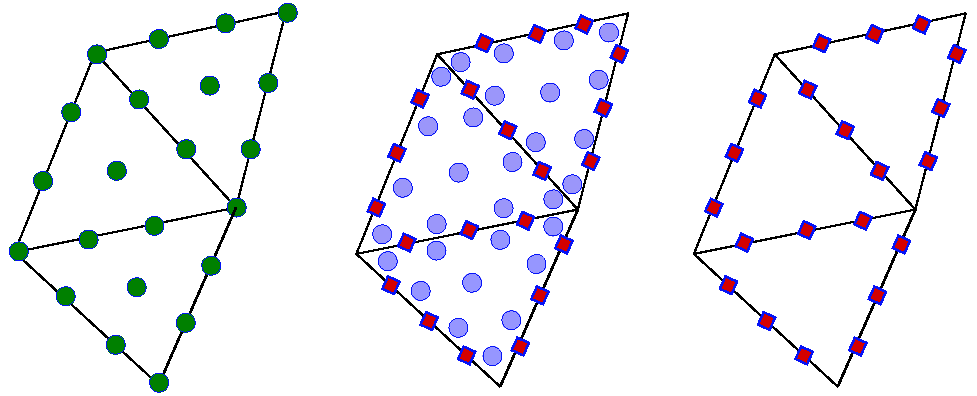
\includegraphics[width=0.55\textwidth]{HHO_FEM}
%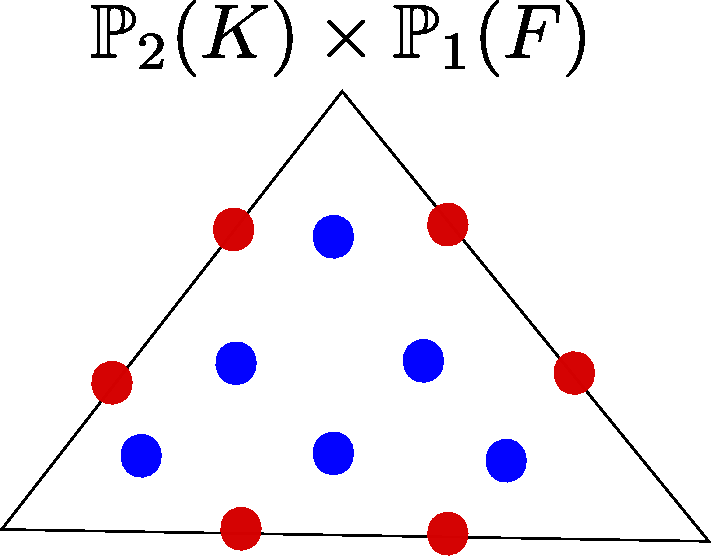
\includegraphics[width=0.32\textwidth]{HHO_P2_P1}
%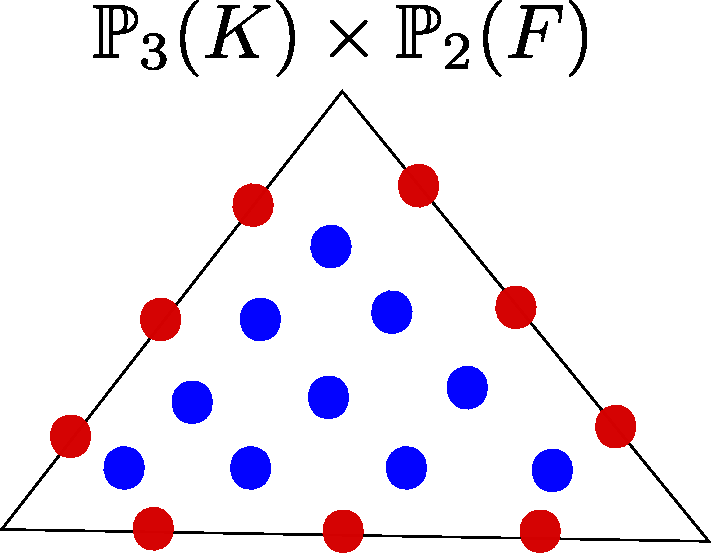
\includegraphics[width=0.32\textwidth]{HHO_P3_P2}
  \end{figure}
  \textcolor{cadmiumgreen}{\textbf{The blue DOFs are eliminated!}}
  
   \scriptsize{ \textcolor{midnightblue}{\textbf{HHO papers:}} Di Pietro, Ern (2015), Cockburn, Di Pietro, Ern (2016), Cascavita, Chouly, Ern (2019), Cicuttin, Ern, Gudi (2020), Chouly, Ern, Pignet (2020)}
\end{frame}
%%%%
\begin{frame}
  \textcolor{cadmiumgreen}{\textbf{Discontinuous spaces:}} \hspace{4 cm} $\Eh$ : \textcolor{midnightblue}{set of edges}, \ $\mathcal{V}_K$ : \textcolor{midnightblue}{DOFs in a triangle}
    \begin{equation*}
    \begin{split}
      X_h^p &:= \prod_{K \in \Th} \mathbb{P}_p(K) \times \prod_{F \in \Eh} \mathbb{P}_{p-1}(F), \quad X_{h,K}^p:= \mathbb{P}_p(K) \times \prod_{F \in \EK} \mathbb{P}_{p-1}(F)\\
      X_{g_{\alpha} h}^p &:= \left\{ v_h \in  X_h^p \ \text{s.t.} \ v_h=g_{\alpha} \ \text{on} \ \partial \Omega \right\}: \ \textcolor{red}{u_1, u_2} \quad \Lambda_h := \prod_{K \in \Th} \mathbb{P}_p(K): \ \textcolor{red}{\lambda}  \\
       \Kghp & := \left\{ \bv_h := \left(v_{1h},v_{2h}  \right) \in X_{g_1 h}^p \times X_{g_2 h}^p \ \text{s.t.} \ \left(v_{1h} - v_{2h}\right)|_{K}(\bx_l) \geq 0 \ \forall \bx_l \in \VK \ \forall K \in \Th \right\}
    \end{split}
    \end{equation*}
    \textcolor{cadmiumgreen}{\textbf{Gradient reconstruction operator in every cell}:} 
$\bG_K : X_{h,K}^p \to \polP_p(K;\R^2)$ such that
\begin{equation*}
  ( \bG_K(\hv_K) , \bq )_{K} \egaldef (\nab v_K , \bq )_K 
  + \sum_{F \in \EK} (v_{F} - v_K , \bq \SCAL \bn_K)_{F} , \quad \forall \hv_K \in X_{h,K}^p, \quad \forall \bq \in \polP_p(K;\R^2),
\end{equation*}
\textcolor{cadmiumgreen}{\textbf{Bilinear form:}} $\forall \hv_h \in X_h^p$, $\forall \hw_h \in X_h^p$
\begin{equation*}
  \begin{split}
  \mathcal{A}_h(\hv_h , \hw_h) \egaldef
  \sum_{K \in \Th} \Big(
  \left(\bG_K(\hv_{K}) , \bG_K(\hw_{K})\right)_{K}
  + h_K^{-1} \sum_{F \in \EK} \left(\Pi_{F}^{p-1}(v_{K} - v_{F}) , w_{K} - w_{F}\right)_{F} 
  \Big) ,
\end{split}
\end{equation*}
\end{frame}
%%%%%%%%%%%
\begin{frame}
        \textcolor{cadmiumgreen}{\textbf{Discrete variational inequality:}} find $\dps \uh=(\uunh,\udeuxh) \in \Kghp$ such that
\begin{equation*}
\dps \sum_{\alpha=1}^2 \mu_{\alpha} \mathcal{A}_h(u_{\alpha h}, v_{\alpha h} - u_{\alpha h}) \geq \sum_{\ialf=1}^2 \sum_{K \in \Th} \left(f_\ialf|_K,v_{\ialf h}|_K-u_{\ialf h}|_K\right)_{K} \quad \forall \bv_h = (v_{1h},v_{2h})\in ~\Kghp \quad \textcolor{electricpurple}{(\mathrm{DR})}
\end{equation*}
  \begin{center}
\textcolor{midnightblue}{Well-posed problem (Lions--Stampacchia)}
\end{center}
  \textcolor{red}{\textbf{HHO without static condensation:}}
  \begin{align*}
\bbE \egaldef 
\left[
  \begin{array}{ccccr}
    \mu_1 \bbS_{CC} 
    & \mu_1 \bbS_{CF} & \bf 0 & \bf 0 & -\mathbb{I}_d 
    \\
    \mu_1 \bbS_{FC} 
    & \mu_1 \bbS_{FF} & \bf 0 & \bf 0 & \bf 0
    \\
    \bf 0 & \bf 0 & \mu_2 \bbS_{CC} & \mu_2 \bbS_{CF} & \mathbb{I}_d
    \\
    \bf 0 & \bf 0 & \mu_2 \bbS_{FC} & \mu_2 \bbS_{FF} & \bf 0
  \end{array}
\right], \quad 
\bF \egaldef \left[\begin{array}{l} \bF_1 \\ \bf 0 \\ \bF_2 \\ \bf 0 \end{array} \right], \quad
%  \\
\X_h \egaldef \left[
  \begin{array}{l}\X_{1h}^{\mathrm{C}}\\ \X_{1h}^{\mathrm{F}} \\ \X_{2h}^{\mathrm{C}}\\ \X_{2h}^{\mathrm{F}} \\ \X_{3h} \end{array} \right] .
  \end{align*}
  \vspace*{-0.2 cm}
  %% \begin{itemize}
  %% \item  $\bF_\alpha \in \mathbb{R}^{m_c}, \ \X_{1h}^{\mathrm{C}} \in \mathbb{R}^{m_c}, \ \X_{2h}^{\mathrm{C}} \in \mathbb{R}^{m_c}, \ \X_{3h} \in \mathbb{R}^{m_c}$, $m_c = \frac{1}{2} (p+1)(p+2) \mathcal{N}_{\mathcal{T}}$
  %% \item $\X_{1h}^{\mathrm{F}} \in \mathbb{R}^{m_F}, \ \X_{2h}^{\mathrm{F}} \in \mathbb{R}^{m_F}$, $m_F := \mathcal{N}_{\varepsilon}^{\mathrm{int}} p$
  %% \end{itemize}
  \invisible<1>{
  \textcolor{red}{\textbf{Discrete complementarity problem}}
\newline
\begin{equation*}
\begin{split}
&\bbE \Xh = \bF,\\
&\textcolor{electricpurple}{\X_{1h}^{\mathrm{C}} - \X_{2h}^{\mathrm{C}}} \geq 0, \quad \textcolor{carmine}{\X_{3h}} \geq 0, \quad \left(\textcolor{electricpurple}{\X_{1h}^{\mathrm{C}} - \X_{2h}^{\mathrm{C}}} \right) \cdot \textcolor{carmine}{\X_{3h}} = 0.
\end{split}
\end{equation*}
\invisible<2>{
  \textcolor{red}{\textbf{Static condensation procedure:}} Later, need the semismooth resolution!
\invisible<3>{
}}}
\end{frame}
%%%%%%%%
\section{Semismooth Newton and first numerical results}
\subsection{}

\begin{frame}
\frametitle{C-functions}
\vspace{-0.2 cm}
\begin{definition}
$f: \left(\R^m\right)^2  \rightarrow \R^m$ ($m \geq 1$) is a
$C$-function or a complementarity function if
\begin{equation*}
\forall(\bx,\by)\in \left(\R^m\right)^2
\qquad f(\bx,\by)=\mathbf{0} \quad \iff \quad
\bx \geq \mathbf{0}, \quad \by \geq \mathbf{0}, \quad \bx {\cdot} \by=0.
\end{equation*}
\end{definition}
\invisible<1>{
\textcolor{cadmiumgreen}{\textbf{min function:}} \ $\left(\min \{\bx, \by\}\right)_l \egaldef \min \left\{\bx_l, \by_l\right\} \qquad l = 1,\dots, m$\\
\vspace{0.2 cm}
\invisible<2>{ \textcolor{cadmiumgreen}{\textbf{ Fischer--Burmeister function:}} \ $\left(f_{\mathrm{FB}}(\bx,\by)\right)_l \egaldef \sqrt{\bx_l^2+\by_l^2}-\left(\bx_l+\by_l\right) \quad  l = 1,\dots, m$
\\ 
\invisible<3>{$\bx=\textcolor{electricpurple}{\X_{1h} - \X_{2h}}$, \ $\by = \textcolor{carmine}{\X_{3h}}$, \ $\CFun(\X_{h})
= \tilde \CFun(\textcolor{electricpurple}{\X_{1h} - \X_{2h}}, \textcolor{carmine}{\X_{3h}})$. 
\begin{equation*}
\left\lbrace\begin{array}{llccc}
\bbE \X_{h} &= \bF,\\
\CFun(\X_{h})&=\mathbf{0}.
\end{array}
\right.
\end{equation*}
\invisible<4>{
\textcolor{red}{\textbf{The C-function is not Fréchet differentiable.}}\\
\vspace{0.2 cm}
\invisible<5>{
\textcolor{red}{\textbf{We will use semismooth Newton algorithms.}} 
\\
\scriptsize{Facchinei and Pang (2003), Bonnans, Gilbert, Lemar\'echal, and Sagastiz\'abal (2006).} 
\invisible<6>{
}}}}}}
\end{frame}
%
\begin{frame}
\frametitle{Inexact semismooth Newton method}
\textcolor{cadmiumgreen}{\textbf{Newton initial vector:}} $\Xh^{\zzero} \egaldef \left(\X_{1h}^{\zzero},\X_{2h}^{\zzero}, \X_{3h}^{\zzero} \right)^{T} \in \R^{3 m}$, on step $\kk \geq 1$, one looks for $\Xh^{\kk} \in \R^{3 m}$ such that
\begin{equation*}
\bbA^{\kk-1}\Xh^{\kk}=\bB^{\kk-1},
\end{equation*} 
where 
\begin{equation*}
\dps \bbA^{\kk-1}\egaldef
\left[\begin{array}{c}
\bbE \\
\JacCFun(\Xh^{\kk-1})
\end{array}
\right],
\quad  \hspace{0.1 cm} \bB^{\kk-1} \egaldef
\left[\begin{array}{c}
\bF\\
\JacCFun(\Xh^{\kk-1})\Xh^{\kk-1}-\CFun(\Xh^{\kk-1})
\end{array}
\right].
\end{equation*}
\textcolor{cadmiumgreen}{\textbf{Inexact solver initial vector:}}
$\Xh^{\kk,\izzero} \in \R^{3 m}$, often taken as $\Xh^{\kk,\izzero} = \Xh^{\kk-1}$, this yields on step $\ii \geq 1$
an approximation $\Xh^{\kk,\ii}$ to $\Xh^{\kk}$ satisfying
\begin{equation*}
\bbA^{\kk-1}\Xh^{\kk,\ii} =\bB^{\kk-1}-{\bm R}_h^{\kk,\ii},
\end{equation*}
where ${\bm R}_h^{\kk,\ii} \in \R^{3 m}$ is the algebraic residual vector.
\end{frame}
%%%%%%
%%%%%%
\begin{frame}
  \frametitle{Newton-min convergence}
  \begin{theorem}
    The Newton-min Algorithm is well defined.
    Moreover, if the first guess $\X_h^0$  is close enough to the solution $\X_h^*$ to the nonlinear system, then the sequence $\left(\Xh^{\kk}\right)_{\kk \geq 1}$ converges to $\X_h^*$ with a finite number of semismooth iterations and the local convergence is quadratic.

    In other words,
    \begin{equation*}
\begin{split}
  \left\| \X_h^{\kk} - \X_h^* \right\|_2 \leq K \left\| \X_h^{\kk-1} - \X_h^* \right\|_2^2,
\end{split}
\end{equation*}
  \end{theorem}

  \end{frame}
%%
\begin{frame}
  \frametitle{HHO with static condensation}
  \begin{itemize}
  \item
  Express the cell components from the face components by local problems
  \item
  By substitution derive from the global system the edge unknowns problem
  \item
  Recover the solution attached to the cells
  \item
  Important computational speed-up 
  \end{itemize}
\begin{table}
  \centering
  \begin{tabular}[h]{| c | c | c | c | c | c | c | c | c |}
    \hline
    &\multicolumn{2}{ c |}{$\polP_1$ DOFs} & \multicolumn{2}{ c |}{$\polP_2$ DOFs} 
    & \multicolumn{2}{ c |}{$\polP_3$ DOFs} & \multicolumn{2}{ c |}{$\polP_4$ DOFs}
    \\
    \hline
    Mesh  & no SC & SC & no SC & SC & no SC & SC & no SC & SC
    \\
    \hline
    $\mathcal{T}_0$   & 752   & 176   & 1504   & 352   & 2448   & 528    & 3584   & 704
    \\
    \hline
    $\mathcal{T}_1$   & 3040  & 736   & 6080   & 1472  & 9888   & 2208   & 14464  & 2944
    \\
    \hline
    $\mathcal{T}_2$ & 12224 & 3008  & 24448  & 6016  & 39744  & 9024   & 58112  & 12032
    \\
    \hline
    $\mathcal{T}_3$ & 49024 & 12160 & 98048  & 24320 & 159360 & 36480  & 232960 & 48640
    \\
    \hline
    $\mathcal{T}_4$ &196352 & 48896 & 392704 & 97792 & 638208 & 146688 & 932864 & 195584
    \\
    \hline
  \end{tabular}
\end{table}  
  \end{frame}
%%%%%%%%%%
\begin{frame}
  \frametitle{Numerical experiments}
  \begin{itemize}
  \item unit square domain $\Omega:=(0,1)\times(0,1)$
  \item We compare the performance of FEM and HHO
  \end{itemize}
  \textcolor{cadmiumgreen}{\textbf{First test case}}
\begin{equation*}
  u_1 (r) \egaldef - u_2(r) \egaldef
  \begin{cases}
    ( r^2 - R^2 )^N 
    &\text{ if } r \geq R ,
    \\
    0 &\text{ otherwise,}
  \end{cases}
  \quad
 \lambda(r) \egaldef
  \begin{cases}
    0 
    &\text{ if } r \geq R ,
    \\
     1000 r^3 (R^2 - r^2)^3 
    &\text{ otherwise,}
  \end{cases}
  \end{equation*}
\begin{itemize}
\item $r \egaldef \sqrt{(x-0.5)^2 + (y-0.5)^2}$ : distance to the center of the domain,
\item $R \egaldef 1/3$: radius of the disk where contact occurs,
\item  $N := 6$
  \end{itemize}
This solution is associated to the right-hand sides $f_1$ and $f_2$ defined by
\begin{align*}
  f_1(r) \egaldef - f_2(r) \egaldef
  \begin{cases}
    -4N (r^2 - R^2)^{N-2} (N r^2 - R^2)
    &\text{ if } r \geq R ,
    \\
    - 1000 r^3 (R^2 - r^2)^3
    &\text{ otherwise.}
  \end{cases}
\end{align*}
\end{frame}
\begin{frame}
 For both schemes, the errors are reported in the energy norm
\begin{equation*}
\tnorm{\bu - \bu_h}_{\Omega} \egaldef \left(\sum_{K\in\Th}\mu_1 \left\|\nab(u_1-u_{1K})  \right\|_{L^2(K)}^2 + \mu_2 \left\|\nab(u_2-u_{2K})  \right\|_{L^2(K)}^2  \right)^{\frac{1}{2}} ,
\end{equation*}
\begin{figure}
\centering
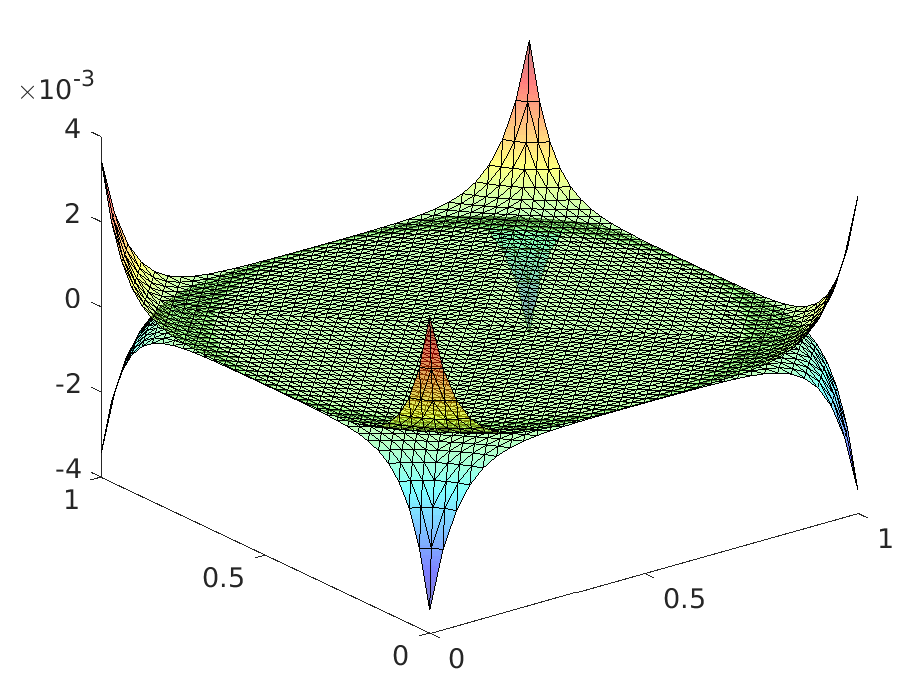
\includegraphics[width=0.48\textwidth]{P2_membrane_cv_J6} \quad
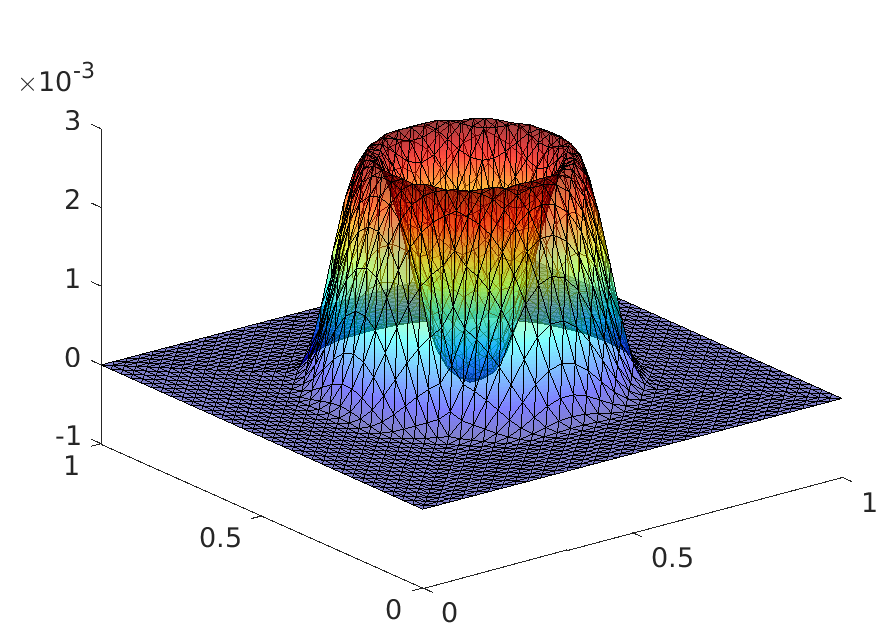
\includegraphics[width=0.48\textwidth]{P2_lambda_cv_J6}
\end{figure}
\end{frame}

\begin{frame}
  \textcolor{red}{\textbf{Number of Newton-min iterations}}
  \vspace*{0.3 cm}
\begin{figure}
\centering
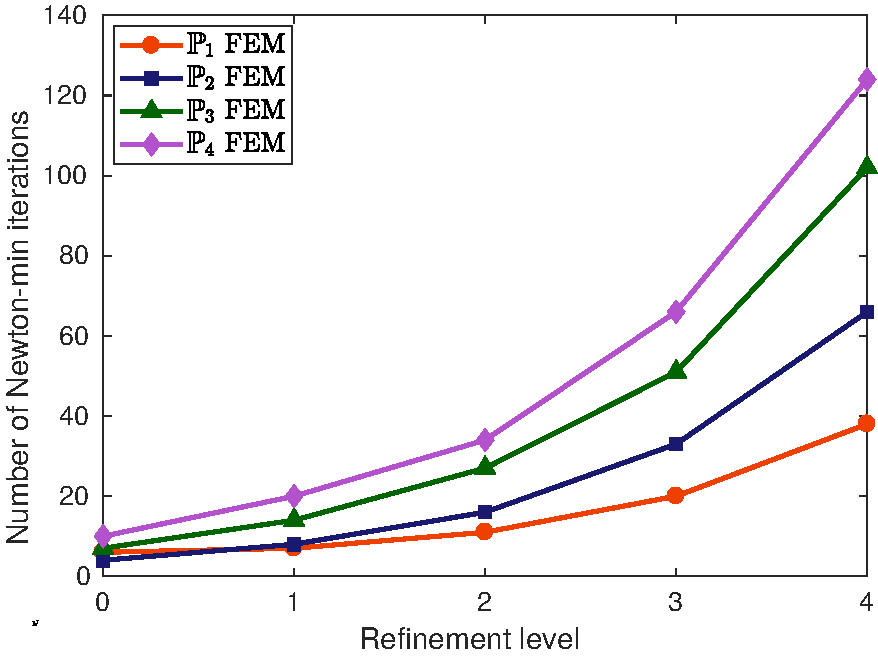
\includegraphics[width=0.48\textwidth]{Number_of_Newton_iter_refinment_level} \quad
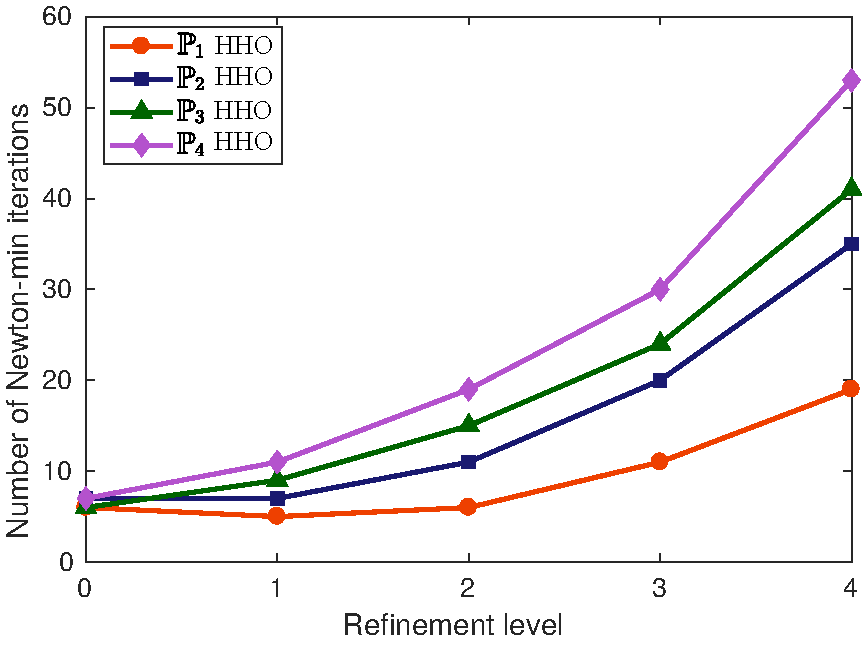
\includegraphics[width=0.48\textwidth]{nb_iter_Newton_HH0}
\end{figure}
  \end{frame}
%%%%%
\begin{frame}
\textcolor{red}{\textbf{Convergence}}
  \begin{figure}
\centering
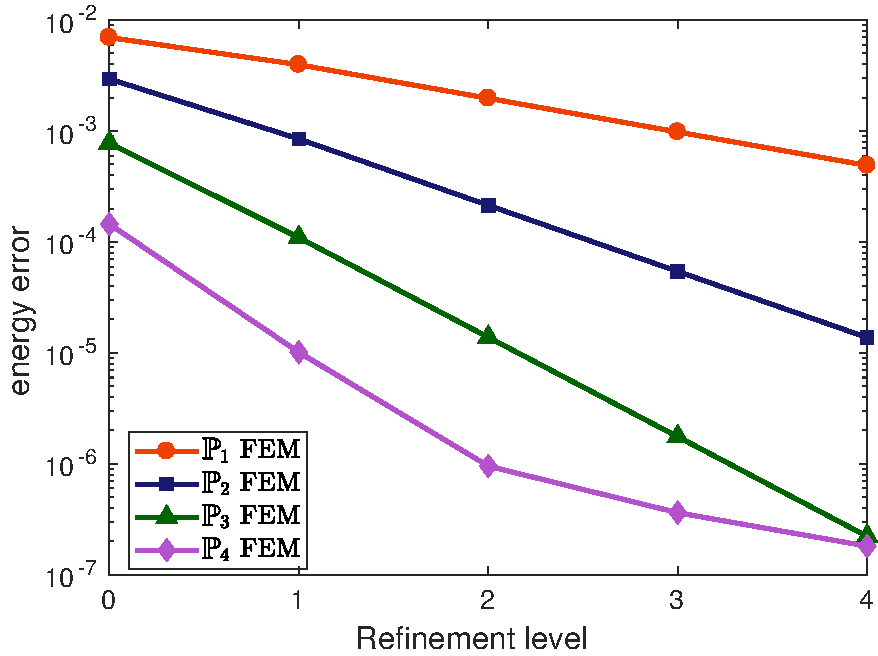
\includegraphics[width=0.48\textwidth]{energy_error_FEM} \quad
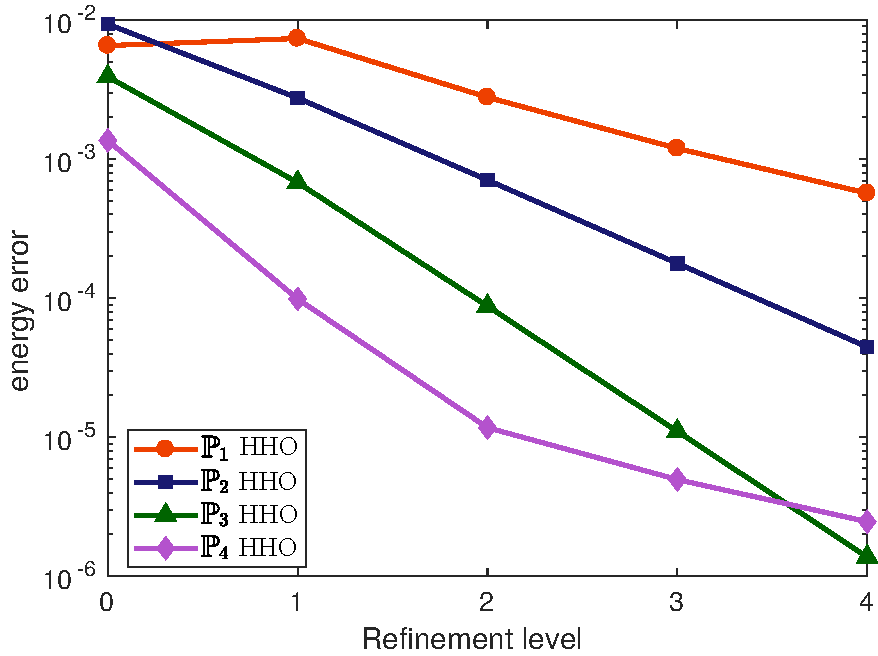
\includegraphics[width=0.48\textwidth]{energy_error_HHO}
\end{figure}
  \end{frame}
\begin{frame}
  \textcolor{cadmiumgreen}{\textbf{A second test case}}
  \begin{align*}
  u_1(r) 
  &\egaldef 
    \begin{cases}
      0 & \text{if } r \leq R ,
      \\
      (r^2 - R^2)^2 &\text{if } r > R ,
    \end{cases}
  %\\
  \quad
  u_2(r) 
  \egaldef 0 ,
\quad
\lambda(r) \egaldef
\begin{cases}
 \dps 1 & \mbox{if } r \leq R,\\
\dps 0 &\mbox{if } r > R,\\
\end{cases}
\end{align*}
This solution is associated to the right-hand sides $f_1$ and $f_2$ given by
\begin{align*}
f_1(r) \egaldef
\begin{cases}
\dps - 8 R^2  &\hspace*{-0.5em}\mbox{if } r \leq R,\\
\dps 8 R^2 - 16 r^2  &\hspace*{-0.5em}\mbox{if } r > R,\\
\end{cases}
\quad
f_2(r) \egaldef
\begin{cases}
\dps 8 R^2 &\hspace*{-0.5em}\mbox{if } r \leq R,\\
\dps 0
&\hspace*{-0.5em}\mbox{if } r > R.\\
\end{cases}
\end{align*}
\vspace*{-0.6 cm}
\begin{figure}
\centering
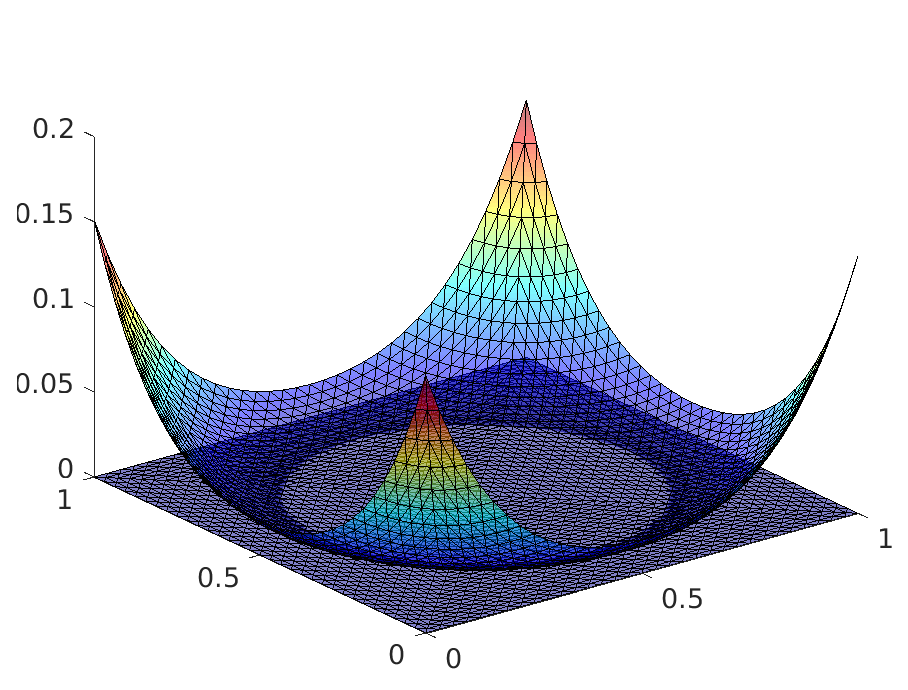
\includegraphics[width=0.40\textwidth]{membrane_P2} \qquad \qquad
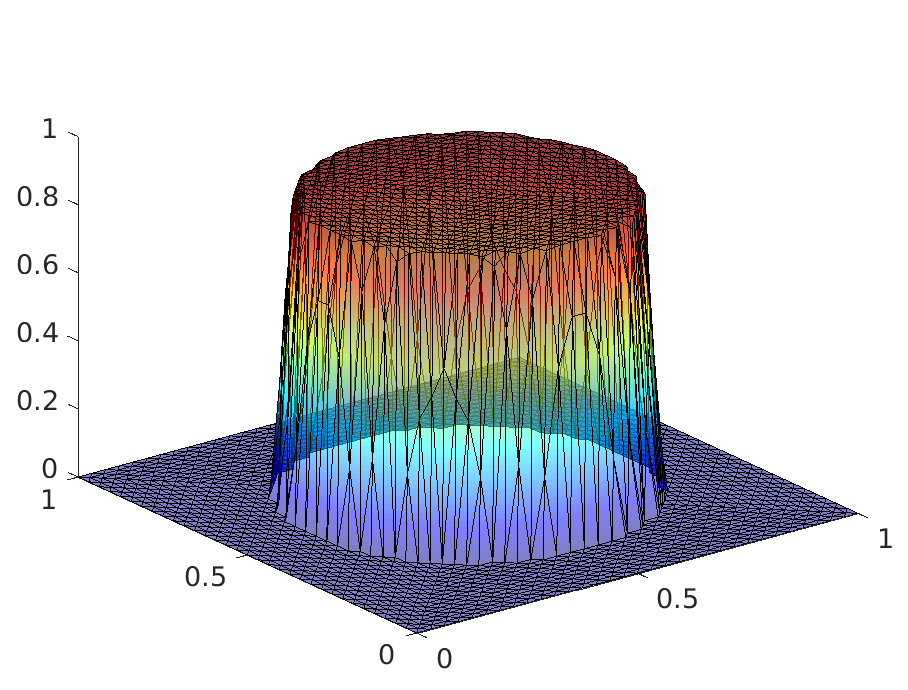
\includegraphics[width=0.40\textwidth]{Lambda_P2}
\end{figure}
\end{frame}

\begin{frame}
  \textcolor{red}{\textbf{Number of Newton-min iterations}}
  \vspace*{0.3 cm}
  \begin{figure}
\centering
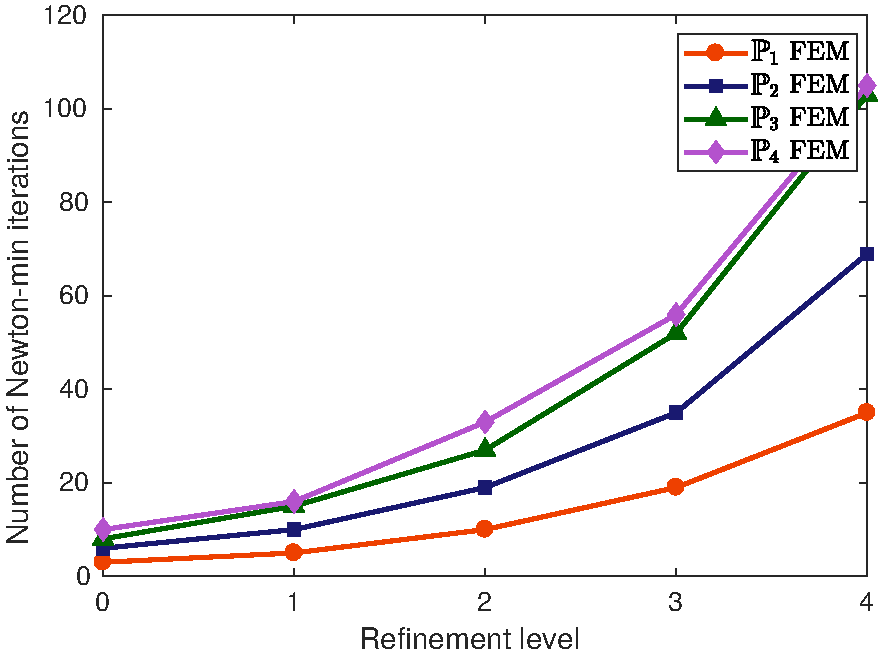
\includegraphics[width=0.48\textwidth]{number_newton_iter_FEM_2nd} \quad
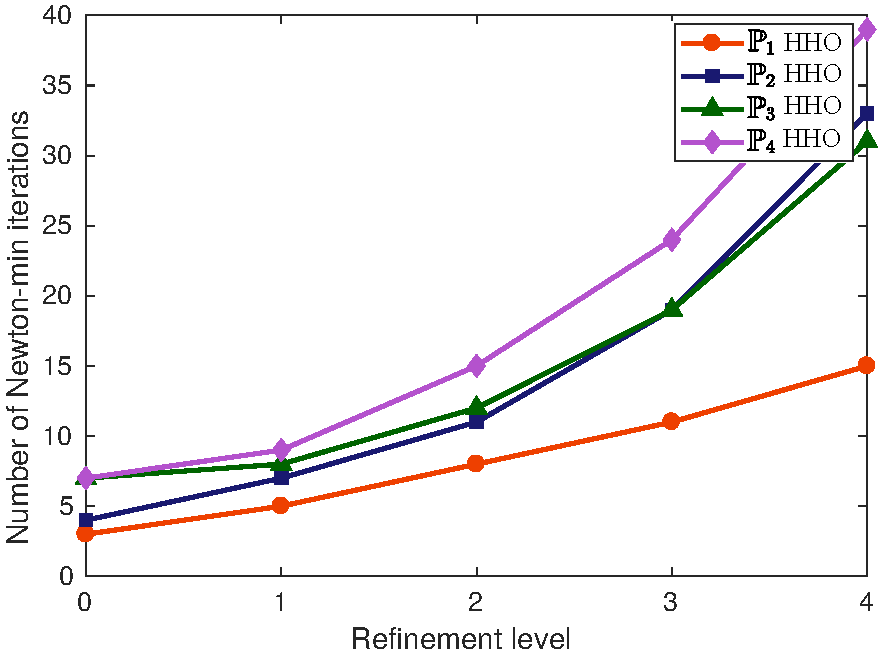
\includegraphics[width=0.48\textwidth]{jump_nb_iter_Newton_HHO}
\end{figure}
  \end{frame}
%%%%%%%%%%%%%%
\begin{frame}
  \textcolor{red}{\textbf{Convergence}}
  \vspace*{0.3 cm}
  \begin{figure}
\centering
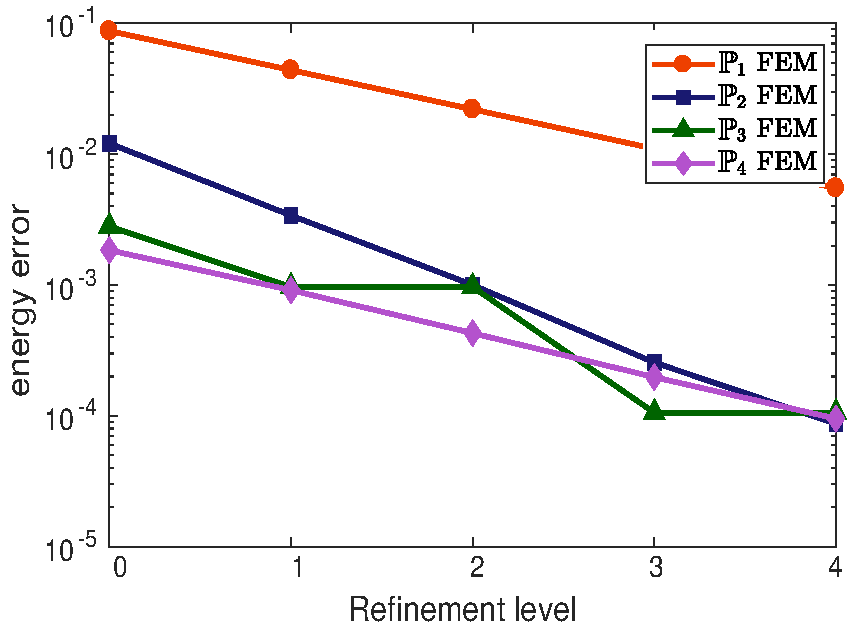
\includegraphics[width=0.48\textwidth]{energy_error_2nd.pdf} \quad
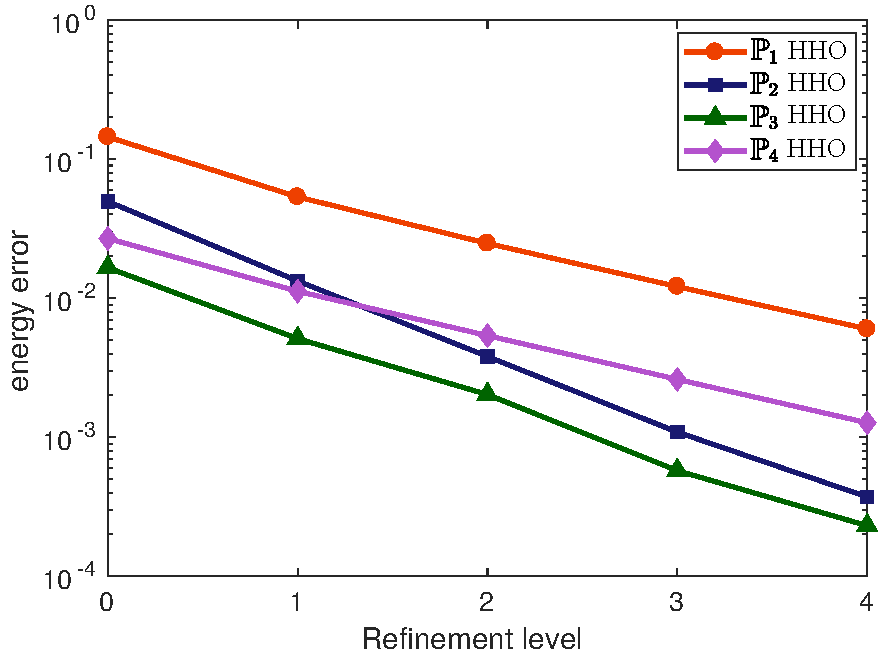
\includegraphics[width=0.48\textwidth]{jump_energy_error_HHO}
  \end{figure}
  \begin{thebibliography}{10}
 \scriptsize{
 \bibitem{Dabaghi:Delay:2020}
 {\sc J.~Dabaghi, G.~Delay}, A unified framework for high-order numerical
discretizations of variational inequalities.
\em{Submitted in Computers \& Mathematics with Applications} (2020).
https ://hal.archives-ouvertes.fr/hal-02969793v1
}
 \end{thebibliography}
\end{frame}
